\documentclass[12pt,a4paper]{report}

\usepackage{geometry}
\usepackage{graphicx}
\usepackage{longtable}
\usepackage{pgfgantt}
\usepackage[dutch]{babel}
\usepackage{url}
\usepackage{pgf,pgfplots}
\usetikzlibrary{fit,calc}
\usepgfplotslibrary{external}

\geometry{a4paper}

\newcommand{\boxplot}[6]{%
	%#1: center, #2: median, #3: 1/4 quartile, #4: 3/4 quartile, #5: min, #6: max
	\filldraw[fill=white,line width=0.2mm] let \n{boxxl}={#1-0.1}, \n{boxxr}={#1+0.1} in (axis cs:\n{boxxl},#3) rectangle (axis cs:\n{boxxr},#4);   % draw the box
	\draw[line width=0.2mm, color=red] let \n{boxxl}={#1-0.1}, \n{boxxr}={#1+0.1} in (axis cs:\n{boxxl},#2) -- (axis cs:\n{boxxr},#2);             	% median
	\draw[line width=0.2mm] (axis cs:#1,#4) -- (axis cs:#1,#6);                                                                           							% bar up
	\draw[line width=0.2mm] let \n{whiskerl}={#1-0.025}, \n{whiskerr}={#1+0.025} in (axis cs:\n{whiskerl},#6) -- (axis cs:\n{whiskerr},#6);        % upper quartile
	\draw[line width=0.2mm] (axis cs:#1,#3) -- (axis cs:#1,#5);                                                                           							% bar down
	\draw[line width=0.2mm] let \n{whiskerl}={#1-0.025}, \n{whiskerr}={#1+0.025} in (axis cs:\n{whiskerl},#5) -- (axis cs:\n{whiskerr},#5);        % lower quartile
}


\begin{document}

%  Titelblad

\begin{titlepage}

\fontsize{12pt}{14pt}\selectfont

\begin{center}

\vspace{1cm}

\fontsize{14pt}{17pt}\selectfont
% De Faculteit:
\textsc{P\&O Computerwetenschappen - Verslag \\Team Platinum}
\fontsize{12pt}{14pt}\selectfont
\vspace{0.3cm}

\vspace{1.2cm}

%Het academiejaar: aanpassen!
Academiejaar 2011--2012

\vspace{2.8cm}

\fontsize{17.28pt}{21pt}\selectfont

% De titel van de thesis:
{\textsc{Pac-Man in de echte wereld,\\ met behulp van Lego Mindstorms}}

\fontseries{m}
\fontsize{12pt}{14pt}\selectfont

\vspace{2cm}


\includegraphics[height=10cm]{resources/Logo-Kul}

\end{center}
\end{titlepage}

\thispagestyle{empty}

\tableofcontents

\begin{abstract}
Tijdens de uitwerking van dit jaar-overschrijdend groepswerk, bouwen wij een autonome robot met behulp van Lego Mindstorms. Voor de programmatie wordt beroep gedaan op Lejos, een Open Bron project dat een minimale JAVA virtuele machine heeft gemaakt die de plaats kan innemen van de standaard programmatie omgeving van Lego.

Naast de doelstelling om kennis te maken met het ontwikkelen van een autonome robot, willen we in dit project ook ervaring opdoen ivm het werken in team verband aan een middelgroot softwareproject. Hierbij zijn organisatie van werk, planning, analyse, architectuur,... belangrijke begrippen.

In het tweede semester wordt hier nog eens de nood aan samenwerking toegevoegd. Het traject van de autonome robot blijft behouden, maar de verschillende robots zullen nu moeten samen werking om een gemeenschappelijk doel te bereiken. Om deze samenwerking in goede banen te leiden werd een scheidsrechtercommissie in het leven geroepen om de beslissingen te nemen die voor alle teams van belang zijn. Het doel van dit semester ligt in het insluiten van een ``Pac-Man''-robot bestuurd door het didactisch team, dit met behulp van vier autonome ``ghosts''.

In het eerste semester werkten we reeds in een parallel traject aan een simulatieomgeving. Aan de hand van deze omgeving waren we in staat om met meerdere teamleden in parallel een robot te ontwikkelen zonder nood aan een fysieke. Nu is het ontwikkelen van deze simulator deel geworden van de verdere opdracht en dienen we dus de nodige aanpassingen te doen om het Pac-Man-spel in de computer te simuleren. Het gebruik van een simulator is evident, aangezien we niet kunnen verwachten alle fysieke testen uit te voeren met de 4 teams tegelijk.
\end{abstract}

\chapter{Inleiding}

Het project wordt zoals in het eerste semester begeleidt door het gebruik van tussentijdse demo's. Het finale doel is om zo optimaal mogelijk samen te werken met vier teams om de Pac-Man in te sluiten, hoewel we ten alle tijden autonoom beslissingen nemen.

Het doel van de eerste demo is een versimpelde vorm van het einddoel waarbij we een stilstaande Pac-Man zoeken binnen het doolhof. De simulator dient ook reeds beschikbaar te zijn. Voor de tweede demo mag de comissie beslissen welke doelstellingen passen in het verdere proces richting het einddoel.

Duidelijk is dat we er in geslaagd zijn om zeer herbruikbare code te produceren in het eerste semester. Iedereen is ondertussen vertrouwd geraakt met de volledige architectuur. Aangezien we duidelijk te maken hebben met een grote diversiteit aan kleine taken, gebeurt het grootste deel van de taakverdeling week op week.

Het verslag is duidelijk verschillend opgebouwd ten opzichte van het vorige semester en kiest voor een onderverdeling in subsecties per demo binnen een context van hoofdstukken. De opbouw van deze hoofdstukken is duidelijk erg gelijkend hoewel natuurlijk de inhoud verandert is tov het eerste semester. Nieuw zijn natuurlijk de stukken over de strategie ivm de opgegeven spelomgeving, over de samenwerking en over de finale analyse van het jaarproject.

\chapter{Probleemstelling}

De doelstellingen van de demo's worden hier achtereenvolgens beschreven, zij liggen in de lijn van het ontwerpproces richting een autonome ghost, die samen met de drie anderen probeert de Pac-Man in te sluiten.

\section{Demo 1}

Het probleem dat we eerst aanpakken is het zo efficient mogelijk in kaart brengen van een onbekende omgeving met behulp van de vier ghosts, belangrijk hierbij is dat de in beeld gebrachte wereld overeenkomt met de realiteit. Tijdens de demo gebruiken we een hybride simulator, onze eigen robot bestaat in de fysieke wereld, de andere drie zijn virtueel en wordt vertegenwoordigd door drie aparte instanties van de simulator, elk met zijn eigen virtuele ``gehost''.

De ``ghosts'' hebben geen enkele informatie over het doolhof waarin ze zich bevinden, noch over hun positie, noch over hun ori\"entatie.. Verder staat de Pac-Man stil in het parcours en dient hij enkel gevonden te worden. We dienen ook aan te tonen dat het door de commissie afgesproken communicatieprotocol ge\"implementeerd is.

Elk team wordt tijdens de demo afzonderlijk beoordeeld.
 
\section{Demo 2}
 
Dit dient nog afgesproken te worden door de commissie.

\section{Demo 3}

\subsection{Verkenning}

De robots rijden in een op voorhand onbekend doolhof. Alle info die verzameld wordt door de vier ghosts draagt bij tot het cre\"eren van een individuele map die mogelijk inconsistenties bevat. Alle juiste info over het doolhof zal direct bijdragen tot het hoofddoel, namelijk het vangen van de pac-man. Elke robot communiceert zijn gevonden informatie en probeert zo veel mogelijk informatie te verzamelen over de rond hem onbekende wereld, het falen van \'e\'en van de robots kan reeds fataal zijn voor het snel kunnen opbouwen van een verkende omgeving. We proberen dus een zo robuust mogelijke robot te maken die zo effici\"ent mogelijk zijn eigen info verzameld en met de nodige voorzichtigheid andere informatie hierin verwerkt.

\subsection{Pac-Man}

Het Pac-Man spel zelf kunnen we winnen door alle vluchtwegen van de Pac-Man af te sluiten. Dit houdt in dat alle omliggende sectoren door een ghost bezet wordt of afgeschermd worden door een muur. Men wint enkel als alle robots die meewerken aan de insluiting ook effectief aangeven dat ze gewonnen hebben via hun grafische interface. De probleemstelling vereist dus een effectieve samenwerking, waarbij een consensus moet bereikt worden over de verzamelde informatie en de te volgen strategie.

\chapter{Scheidsrechtercomissie}

Deze commissie staat in voor het nemen van beslissingen die betrekking hebben op afspraken tussen de verschillende teams en het didactische team. Hierbij kunnen we deze beslissingen groeperen in:
\begin{itemize}
	\item De verdere regels waarmee de spelomgeving beperkt wordt.
	\item Afspraken die noodzakelijk zijn voor de samenwerking van de teams.
\end{itemize}

\section{Spelregels}

\subsection{SpelWereld}

De spelwereld bestaat uit aangepaste panelen uit het eerste semester. Er is een raster van witte lijnen ge\"introduceerd waar mogelijks muren kunnen staan. Dit komt neer op een mogelijke herschaling van de panelen met een factor vier. Deze nieuwe minimumeenheid aan oppervlakte noemen we sectoren. Deze zijn belangrijk voor de plaatsbepaling binnen het doolhof. De doolhof is volledig ommuurd en de absolute afmetingen worden op voorhand gegeven.

\subsection{Pac-Man}

De Pac-Man wordt zichbaar gemaakt door een infrarood-beacon dat kan opgemerkt worden met behulp van de voorziene IR-sensor. Het didactisch team kiest waar deze vertrekt en bestuurt hem tijdens de demo's. Hij mag enkel bewegen op sectoren waar zich geen ``ghosts'' beevinden.

De beweging van Pac-Man is beperkt tot het rechtdoor oversteken van de witte lijnen die de sectoren scheiden.

\subsection{Ghosts}

De ghosts vertrekken op de vier hoekpunten van de doolhof, zodat de verkenning van de doolhof zo snel mogelijk van start kan gaan. De orientatie van de robot is onbekend hoewel de hoek tov het assenstel wel een veelvoud is van 90 graden.


\section{CommunicatieProtocol}

Te vinden in pdf.
\subsection{Voordelen}

\subsection{Nadelen}


\chapter{Robot}

\section{Demo 1}

\subsection{Fysiek ontwerp}

Door de veranderde specificaties van het doolhof en de extra infrarood sensor, moesten enkele wijzigingen gemaakt worden aan de fysieke robot. Zo zijn de druksensoren verwijderd om een sensor poort vrij te maken voor de infrarood sensor. Verder werd de hoogte van de robot iets verlaagd door het verplaatsen van de motor die verantwoordelijk is voor het draaien van de sonar. Naast een grotere stabiliteit doordat het zwaartepunt van de robot lager bij de grond ligt staat ook de motor stabieler, waardoor nauwkeurigere metingen mogelijk zijn. (ALS WE DIT LATEN STAAN, DAN GAAN ZE VRAGEN NAAR NUMERIEKE ONDERSTEUNING VAN DIE OPMERKING) Aangezien het doolhof minder breed is (sectoren zijn 40 centimeter in plaats van 80) zijn de extra wielen weggehaald om het geheel iets slanker te maken wat een eenvoudigere navigatie mogelijk maakt.

\subsection{Testen}

Ir Sensor

\section{Demo 2}

\section{Demo 3}

\chapter{Strategie}

\section{Strategie van Robot}

Aangezien wij ons slechts sinds enkele maanden begeven op het terrein van autonome robots en artifici\"ele intelligentie, zou het dom zijn te veronderstellen dat er ons nog niemand is voor gegaan. We hebben daarom een literatuurstudie rond de concepten van Pac-Man en autonome ``ghosts'' gedaan.

We vonden een paper omtrent ``Collaborate Diffusion''\footnote{http://www.cs.colorado.edu/~ralex/papers/PDF/OOPSLA06antiobjects.pdf}. Hierin wordt voorgesteld om een vorm van ``Hill Climbing'' \footnote{http://en.wikipedia.org/wiki/Hill\_climbing/} toe te passen om zo verschillende autonome ``ghosts'' toe te laten samen te werken om een ``Pac-Man'' te achtervolgen. Hierbij hebben zij geen nood aan bijkomende onderlinge communicatie naast de informatie over de wereld.

Ondanks het feit dat we geen overeenstemming met de andere teams konden bereiken om allen dit algoritme te implementeren, blijft het een zeer interessant algoritme om toe te passen voor het bepalen van ons eigen pad.

\subsection{Achtervolgstrategie}

Wanneer de Pac-Man gezien wordt stuurt deze een ``geur'' uit. Deze plant zich langs gekende sectoren voort. Dit wordt gedaan door het gemiddelde van de 4 omliggende sectoren te berekenen, indien er een muur staat is de waarde 0. Zo ontstaat er een hoogte-kaart met aan de top een Pac-Man. De Ghosts kunnen nu aan de hand van een eenvoudig ``Hill Climbing'' algoritme een optimale weg volgen naar de Pac-Man.

Wanneer een ``ghost'' de Pac-Man opmerkt, kan deze positie op de kaart een zeer hoge waarde gegeven worden. Deze kaart wordt vaak herberekend en de geur van een Pac-Man zal dus snel verdwijnen. En dit is zoals het in de realiteit ook zal zijn. De Pac-Man beweegt zich doorheen het doolhof en zal niet op \'e\'en plek blijven wachten. Als een Pac-Man meerdere keren gezien wordt zal zijn positie ook een constantere ``geur'' verspreiden, waardoor de ``ghosts'' van alle kanten op hem kunnen naderen. Figuur \ref{fig:hillclimbing1} toont het principe aan de hand van een visualisatie van de hoogte of geur van de Pac-Man door middel van een kleurenpallet. Hierbij zijn hoge waarden rood gekleurd en lage waarden violet.

\begin{figure}[htbp]
  \centering
  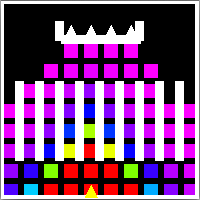
\includegraphics[width=50mm]{resources/hillclimbing1.png}
  \caption{Hill Climbing}
  \label{fig:hillclimbing1}
\end{figure}

Om te voorkomen dat robots allemaal dezelfde weg volgen en enkel achter Pac-Man lopen slorpt iedere Ghost de geur op door de waarde van zijn huidig vakje op 0 te zetten. Hierdoor ontstaat er een dal rond iedere Ghost en zullen de anderen een omweg zoeken. Dit zorgt er ook voor dat de Ghosts elkaar van nature uit ontwijken en niet zullen botsen. Figuur \ref{fig:hillclimbing2} illustreert dat, eens een Ghost een bepaalde ``beste'' route naar de Pac-Man heeft ingeslagen, het pad achter hem minder interessant wordt voor de overige achtervolgers.

\begin{figure}[htbp]
  \centering
  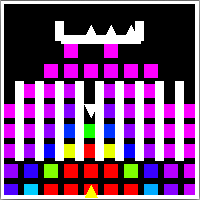
\includegraphics[width=50mm]{resources/hillclimbing2.png}
  \caption{Hill Climbing met afsluiting van pad}
  \label{fig:hillclimbing2}
\end{figure}

\subsection{Verkenstrategie}

De verkenstrategie is gebaseerd op het zelfde principe. Hier is er niet \'e\'en bron die een geur uitstuurt, maar iedere onbekende sector stuurt een geur uit. De robot zal hierdoor altijd naar het dichtstbijzijnde en het meest onverkende stuk van het doolhof willen gaan. Daarnaast zorgt dit principe er ook voor dat een robot zal terugkeren op zijn stappen en automatisch terugkeert naar achtergelaten onbekende sectoren. We kunnen stellen dat het algoritme impliciet ``Depth-First-Search"\footnote{http://en.wikipedia.org/wiki/Depth-first\_search} implementeert. Figuur \ref{fig:dfs} toont een robot die een onbekend doolhof aan het verkennen is. De fel groene sectoren zijn onbekende sectoren en hebben een hogere waarde dan de reeds bezochte sectoren.

\begin{figure}[htbp]
  \centering
  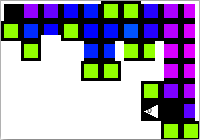
\includegraphics[width=50mm]{resources/dfs.png}
  \caption{Hill Climbing met impliciet ``Dept-First-Search'' zoekgedrag}
  \label{fig:dfs}
\end{figure}

Het toepassen van het zelfde algoritme voor beide deelproblemen, levert ons in essentie een enkelvoudige implementatie van beide. Door het toekennen van goed gekozen waarden aan onbekende sectoren en aan sectoren waar Pac-Man werd gezien, stelt het algoritme ons in staat om steeds het optimale doel te kiezen. Wanneer er zich geen pad bevindt naar de Pac-Man zal een ``ghost'' onbekende sectoren trachten te verkennen. Wanneer er een pad bestaat naar de Pac-Man zal zijn ``geur'' dit pad nog extra versterken en zal een ``ghost'' automatisch hierdoor aangetrokken worden.

\chapter{SoftwareDesign}
\section{Demo 1}
\subsection{Robot}
\subsection{PC}
\section{Demo 2}
\section{Demo 3}


\chapter{Simulator}
\section{Demo 1}
\subsection{Virtualisatie}
\subsection{Granulariteit}
\subsection{Testen}
\section{Demo 2}
\section{Demo 3}

\chapter{Conclusies}
\section{Demo 1}
\section{Demo 2}
\section{Demo 3}
\chapter{Procesbeschrijving}

\chapter{Werkverdeling}

\begin{longtable}{l l}
\caption{Focus van elk team lid} \\ [0.5ex]
%This is the header for the first page of the table...
\hline\hline
Teamlid & Focus \\ [0.5ex]
\hline 
\endfirsthead
%This is the header for the remaining page(s) of the table...
\multicolumn{2}{c}{{\tablename} \thetable{} -- Vervolg} \\[0.5ex]
\hline \hline
Teamlid & Focus \\ [0.5ex]
\hline 
\endhead
Michiel 		& 	(Commissie-lid) GhostRobot. \\
Florian 		&	\\
Ruben 		&	IR-sensor, Simulator.\\
Thomas 		&	\\
Daniel 		&	\\
Christophe 	&	Diffusion algoritme, Dashboard \\
\hline
\label{tab:focus}
\end{longtable}

\begin{longtable}{l r r r r r r r}
\caption{Tijdsbesteding per team lid per week} \\
%This is the header for the first page of the table...
\hline\hline
 & michiel & florian & ruben & thomas & daniel & christophe & totaal \\
\hline 
\endfirsthead
totaal & 61 & 19 & 43 & 36 & 13 & 63 & 235\\
\hline
week 1 & 12 & 9 & 13 & 12 & 0 & 16,5 & 62,5 \\
week 2 & 16,5 & 5 & 14 & 15 & 8 & 17,5 & 76 \\
week 3 & 32,5 & 5 & 16 & 9 & 5 & 29 & 96,5 \\
\hline
gemid./week & 20 & 6 & 14 & 12 & 4 & 21 & 13 \\
\label{tab:tijdsregistratie}
\end{longtable}

In samenspraak met het didactische team, zal Christophe gedurende twee van de vijf uren die standaard ingepland staan op maandag het team niet vervoegen. Deze uren worden enerzijds onmiddellijk voorafgaandelijk alsook 's avonds na deze vaste uren gepresteerd.

\chapter{KritischeAnalyse}

Dit deel wordt later toegevoegd.

\appendix

\chapter{Beoordelingen}

\chapter{Grafische User Interface}

\chapter{Klasse Diagrammen}


\chapter{Planning}
\label{appendix:planning}

\begin{figure}[htbp]
\centering
\begin{tikzpicture}
	\begin{ganttchart}[ 
	  y unit title=0.6cm,
	  y unit chart=0.5cm,
	  vgrid,
	  bar height=.5,
	  group right shift=0,
	  group top shift=.6,
	  group height=.3]{22}
\gantttitle{Oktober}{10} 	   	\gantttitle{November}{8} 	    \gantttitle{December}{4} \\
\gantttitlelist{3,10,17,24,31}{2}	\gantttitlelist{7,14,21,28}{2}  \gantttitlelist{5,12}{2} \\
\ganttgroup{1. Beweging}{1}{5} \\
\ganttbar{1.1. API Tijd}{2}{4} \\
\ganttbar{1.2. API Omw.}{2}{4} \\
\ganttbar{1.3. Tijd}{4}{5} \\
\ganttbar{1.4. Omw.}{4}{5} \\
\ganttbar{1.5. tests}{5}{5} \\
\ganttbar{2. Veelhoek}{3}{5} \\
\ganttbar{3. LCD}{2}{5} \\
\ganttmilestone{Demo 1}{5} \ganttnewline
\ganttgroup{4. Verslag}{1}{20} \\
\ganttbar{4.1. Demo 1}{2}{5} \\
\ganttbar{4.2. Demo 2}{8}{12} \\
\ganttbar{4.3. Finaal}{18}{20} \\
\ganttgroup{5. Comm.}{3}{20} \\
\ganttgroup{5.1. Robot}{3}{20} \\
\ganttbar{5.1.1. Log}{3}{11} \\
\ganttbar{5.1.2. Commando}{11}{20} \\
\ganttgroup{5.2. PC}{5}{20} \\
\ganttbar{5.2.1. Log}{5}{11} \\
\ganttbar{5.2.2. Commando}{11}{20} \\
\ganttbar{6. Model}{3}{18} \\
\end{ganttchart}
\end{tikzpicture}
\caption{Planning}
\label{fig:planning}
\end{figure}

\begin{figure}[htbp]
\centering
\begin{tikzpicture}
	\begin{ganttchart}[ y unit title=0.6cm, y unit chart=0.5cm,  vgrid,
	  bar height=.5,
	  group right shift=0,
	  group top shift=.6,
	  group height=.3]{22}
\gantttitle{Oktober}{10} 	   	\gantttitle{November}{8} 	    \gantttitle{December}{4} \\
\gantttitlelist{3,10,17,24,31}{2}	\gantttitlelist{7,14,21,28}{2}  \gantttitlelist{5,12}{2} \\
\ganttgroup{7. Navigator}{5}{18} \\
\ganttbar{7.1. Abstract}{5}{11} \\
\ganttbar{7.2. Design}{11}{18} \\
\ganttbar{7.3. Impl.}{13}{18} \\
\ganttbar{7.4. Tests}{15}{18} \\
\ganttbar{8. Simulator}{3}{13} \\
\ganttbar{9. Log server}{5}{11} \\
\ganttbar{10. Syslog}{7}{10} \\
\ganttbar{11. DB server}{7}{10} \\
\ganttgroup{12. Fat client}{9}{16} \\
\ganttbar{12.1. Status}{9}{14} \\
\ganttbar{12.2. Commando}{10}{16} \\
\ganttgroup{13. SOA}{9}{12} \\
\ganttbar{13.1. REST}{9}{11} \\
\ganttbar{13.2. web client}{10}{12} \\
\ganttbar{14. Smart client}{12}{18} \\
\ganttbar{15. Calibratie}{12}{18} \\
\ganttbar{16. Unit tests}{2}{18} \\
\ganttgroup{17. Lijnvolger}{5}{10} \\
\ganttbar{17.1. Onderzoek}{5}{8} \\
\ganttbar{17.2. Sensor}{7}{9} \\
\ganttbar{17.3. Impl.}{9}{10} \\
\ganttgroup{18. Muurvolger}{5}{10} \\
\ganttbar{18.1. Onderzoek}{5}{8} \\
\ganttbar{18.2. Sensor}{7}{9} \\
\ganttbar{18.3. Impl.}{9}{10} \\
\ganttgroup{19. Barcode}{5}{10} \\
\ganttbar{19.1. Onderzoek}{5}{8} \\
\ganttbar{19.2. Detectie}{7}{9} \\
\ganttbar{19.3. Impl.}{9}{10} \\
\ganttmilestone{Demo 2}{10} \ganttnewline
\ganttmilestone{Finale Demo}{18} \ganttnewline
\ganttbar{20. Finaal verslag}{19}{20} \\
\end{ganttchart}
\end{tikzpicture}
\caption{Planning (vervolg)}
\label{fig:planning2}
\end{figure}

\end{document}
